\section{Ecken kompatible Paare}

In diesem Abschnitt werden wir uns mit einer zweiten Charakterisierung von SLTRs auf planaren Graphen nach \cite{af15} beschäftigen, die eine Verbindung zwischen Schnyder Woods und FAAs herstellt und so zu einer hinreichenden Bedingung für SLTRs führt. Zum Einstieg folgt die Definition dieses Zusammenhanges.

\begin{definition}[Ecken Kompatibilität]\label{def_ccc}
Ein Paar $(\sigma,\phi)$ aus einem Schnyder Labeling $\sigma$ und einem FAA $\phi$ nenne wir \textit{Ecken kompatibel}, falls:
\begin{itemize}
\item [C1] Das Schnyder Labeling $\sigma$ und das FAA $\phi$ nutzen die selben Aufhängungen.
\item [C2] In jedem inneren Gebiet haben die drei Ecken aus $\phi$ drei unterschiedliche Label in $\sigma$.
\end{itemize}
\end{definition}

Der Rest dieses Kapitels wird sich mit dem Beweis beschäftigen, dass zu jedem SLTR (mindestens ein) Ecken kompatibles Paar existiert und das anders herum jedes Ecken kompatible Paar eine SLTR induziert.

\begin{theorem}
\label{theo_ccc}
Sei G ein planer, intern-3-zusammenhängender Graph mit den Aufhängungen $\{a_1,a_2,a_3\}$. G besitzt eine SLTR, genau dann wenn ein Ecken kompatibles Paar $(\sigma,\phi)$ aus einem Schnyder Labeling $\sigma$ und einem FAA $\phi$ existiert.
\end{theorem}

Wir beweisen zuerst die (deutlich einfachere) Rückrichtung des Theorems. Hier können wir die durch das in Abschnitt \ref{sw} erklärte \textit{face counting} erhaltene Einbettung nutzen, um zu zeigen, dass jeder begrenzende Zykel $\gamma$ genau drei kombinatorisch konvexe Ecken besitzt. 

\begin{lemma}\label{lem1}
Sei G ein planer, intern-3-zusammenhängender Graph mit den Aufhängungen $\{a_1,a_2,a_3\}$. Falls ein Paar $(\sigma,\phi)$ aus einem Schnyder Labeling $\sigma$ und einem FAA $\phi$ Ecken kompatibel ist, dann hat jeder begrenzende Zykel $\gamma$ genau drei kombinatorisch konvexe Ecken im Bezug auf $\phi$.
\end{lemma}

\begin{proof}
Sei $\gamma$ ein begrenzender Zykel und $F_{in}$ die Menge der inneren Gebiete von $G$. Seien $\alpha_1=(0,1),\alpha_2=(1,0)$ und $\alpha_3=(0,0)$ drei linear unabhängige Vektoren in $\mathbb{R}^2$. $D$ sei die durch \textit{face counting} erhaltende Zeichnung von $G$ mit den Ecken $\alpha_1,\alpha_2,\alpha_3$. Ein Beispiel einer solchen Zeichnung findet sich in Abbildung \ref{face_counting}. Betrachte nun den begrenzenden Zykel $\gamma$ in $D$. Wir schieben nun, wie in Abbildung \ref{sweeplines1} illustriert, ausgehend von $\alpha_i$ die Geraden $(\alpha_{i+1},\alpha_{i-1})$ über den Graphen. Sei $M_i$ die Menge der zuerst von $(\alpha_{i+1},\alpha_{i-1})$ getroffenen Knoten von $\gamma$ für $i \in (1,2,3)$.

\begin{observation}\label{obs1}
Alle Knoten um ein inneres Gebiet $f$ mit Label $i$ in $f$ werden von der Gerade $(\alpha_{i+1},\alpha_{i-1})$ zum gleichen Zeitpunkt getroffen. Dies folgt direkt aus Eigenschaft W5 (Abschnitt \ref{sw}), da alle Knoten mit dem selben Label in der Zeichnung auf $c_i(\alpha_{i+1},\alpha_{i-1})$ platziert werden.
\end{observation}

\begin{observation}\label{obs2}
Sei $v \in M_i$. Alle Winkel an $v$ im Inneren von $\gamma$ haben das Label $i$. Die Geraden teilen die Winkel um einen Knoten (siehe Abbildung \ref{sweeplines2}). Die Winkel an $v$, die von $a_i$ aus gesehen vollständig auf der anderen Seite von $(\alpha_{i+1},\alpha_{i-1})$ liegen, haben Label $i$.
\end{observation}

\begin{figure}
  \centering
  \begin{minipage}{0.4\textwidth}
  \centering
    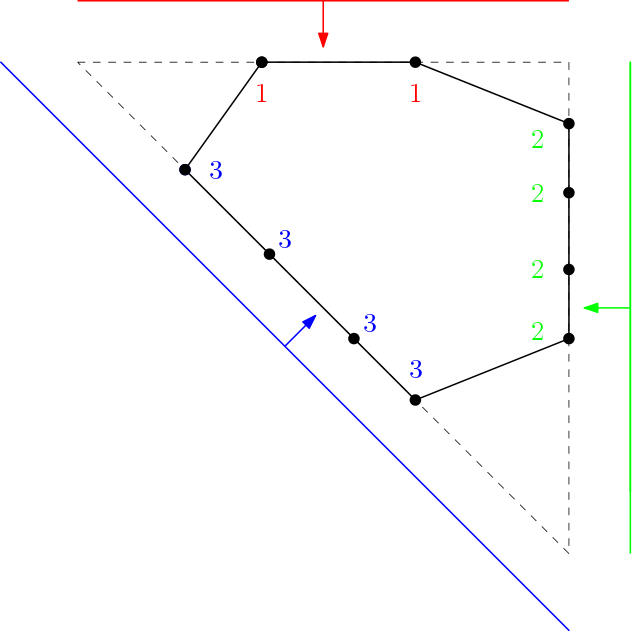
\includegraphics[width=0.9\textwidth]{sweeplines1.png}
    \caption{}
    \label{sweeplines1}
  \end{minipage}
  \hfill
  \begin{minipage}{0.4\textwidth}
  \centering
    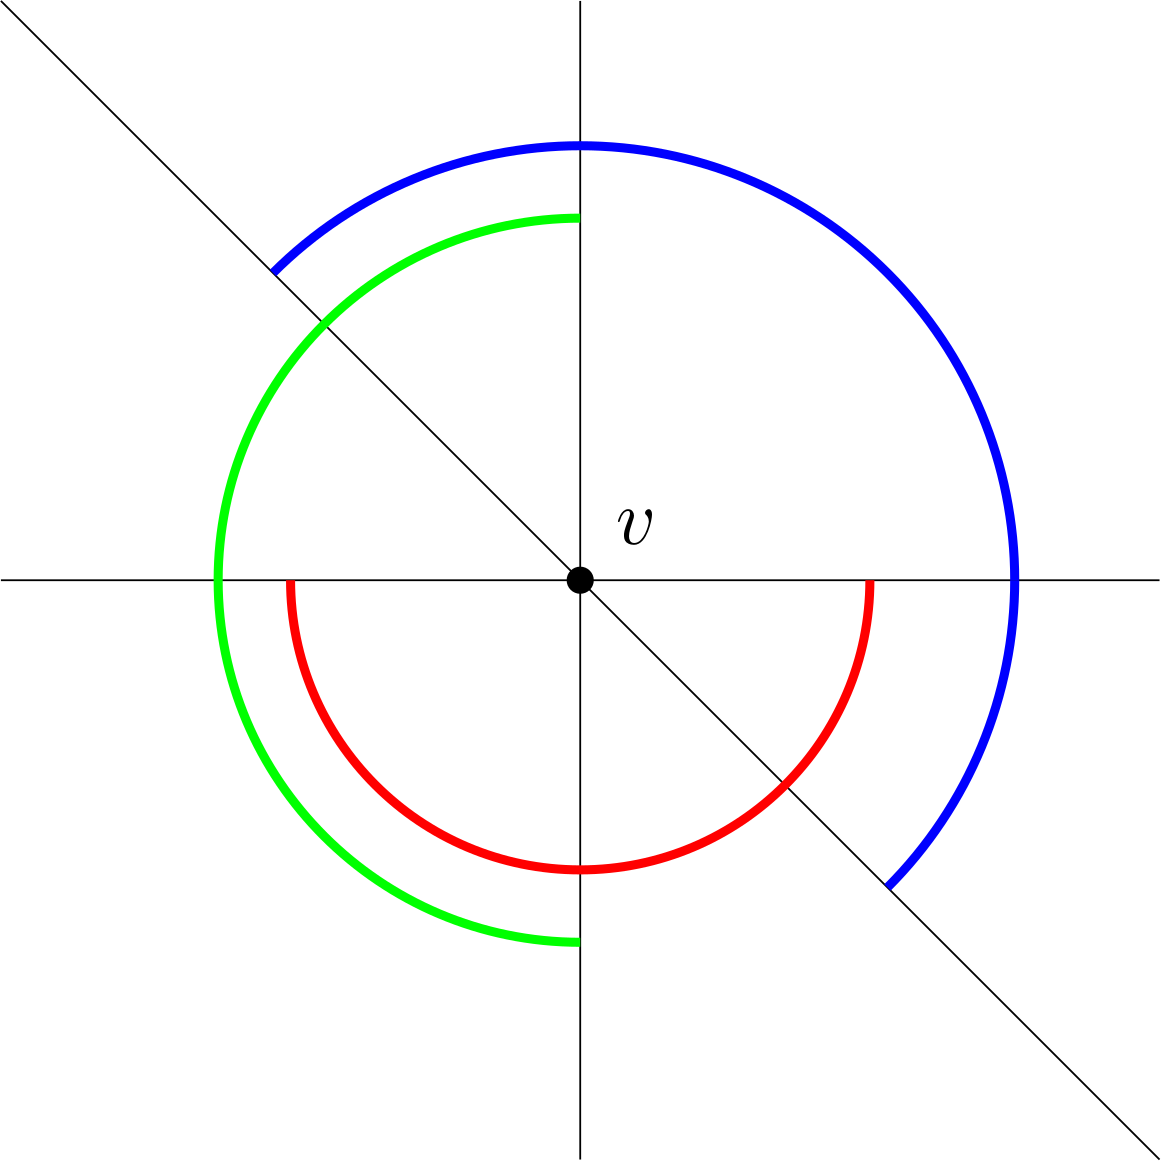
\includegraphics[width=0.9\textwidth]{sweeplines2.png}
    \caption{}
    \label{sweeplines2}
  \end{minipage}
\end{figure}

Nach Beobachtung \ref{obs2} sind die Mengen $M_1,M_2$ und $M_3$ disjunkt. Wir suchen nun nach drei kombinatorisch konvexen Ecken von $\gamma$. Das FAA und das Schnyder Labeling sind Ecken kompatibel und somit hat jedes Gebiet $f \in F_{in}$ einen Winkel mit Label $i$. Also liegt in jeder Menge $M_i$ ein Knoten $v_i$, der vom FAA nicht einem Gebiet innerhalb von $\gamma$ zugewiesen wird. Nehmen wir an $a_i \notin M_i$, denn sonst hätten wir nach E1 eine Ecke gefunden. Da $D$ eine konvexe Zeichnung ist muss $v_i$ einen Nachbarn ausserhalb von $\gamma$ besitzen. Somit liegt $v_i$ auf $\gamma$, ist nicht in $\gamma$ zugewiesen und hat einen Nachbarn ausserhalb von $\gamma$. $v_i$ erfüllt also E2 und somit hat jeder begrenzende Zykel drei kombinatorisch konvexe Ecken (jeweils eine aus jedem $M_i$).
\end{proof}

Zusammen mit Theorem \ref{com_theo} folgt, dass es sich bei dem FAA um ein Gutes-FAA handelt. Somit induziert das Ecken kompatible Paar ein SLTR von $G$.\\

Machen wir uns an den Beweis der Hinrichtung. Zu jedem SLTR können wir ein eindeutiges FAA erstellen indem wir die flachen Winkel der SLTR im FAA zuweisen. Wir müssen also zeigen, dass zu jeder SLTR ein Schnyder Labeling existiert, das zusammen mit dem induzierten FAA ein Ecken kompatibles Paar bildet. Sei $G$ ein planer, intern-3-zusammenhängender Graph mit den Aufhängungen $\{a_1,a_2,a_3\}$, der (mindestens) eine SLTR besitzt. Sei $\Delta$ eine SLTR von $G$ und sei $\phi$ das von $\Delta$ induzierte FAA.

Vor dem nächsten Lemma müssen wir zwei geometrische Objekte einführen. Beispiele finden sich in Abbildung \ref{subdividing_ex}.

\begin{definition}[Unterteilendes Dreieck]
Ein \textit{unterteilendes Dreieck} ist ein Dreieck in der Zeichnung einer SLTR von $G$, sodass gilt:
\begin{itemize}
\item Jeder Knoten auf dem Rand des Dreiecks (der keine Ecke des Dreiecks ist) ist entweder ausserhalb oder innerhalb des Dreiecks zugewiesen
\item Es existiert ein Knoten (der keine Ecke ist), der keine Nachbarn ausserhalb des Dreiecks hat und es existiert ein Knoten (der keine Ecke ist), der keine Nachbarn im Inneren des Dreiecks hat.
\end{itemize}
Dieses Dreieck kann Teile des Randes der Zeichnung beinhalten.
\end{definition}

\begin{definition}[teilendes Segment]
Ein \textit{teilendes Segment} eines SLTR von $G$ ist eine Menge von Kanten $\{e_1, \ldots , e_m\}$, die alle auf einer Gerade liegen, sodass gilt:
\begin{itemize}
\item Die Vereinigung der Kanten trennt die Zeichnung in zwei nichtleere Teile. 
\item Jeder innere Knoten $v$ auf dem Segment ist einem Gebiet zugeordnet, dass zwei Kanten beinhaltet die auf dem Segment liegen. Diese beiden Kanten haben $v$ als Endpunkt.
\end{itemize}
\end{definition}

\begin{figure}[h]
	\centering
	  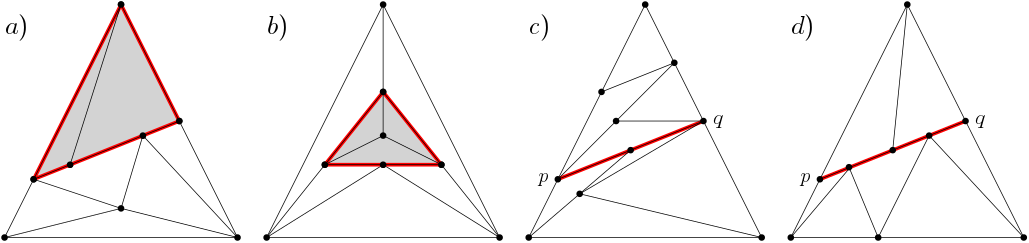
\includegraphics[width=0.9\textwidth]{subdividing_ex.png}
    	\caption{Beispiele von unterteilenden Dreiecken in a) und b) und teilenden Segmenten in c) und d) jeweils in rot.}
    	\label{subdividing_ex}
\end{figure}

Um zu zeigen, dass wir zu jeder SLTR ein passendes Ecken kompatibles Paar $(\sigma,\phi)$ finden führen wir einen Widerspruchsbeweis. Sei $G$, ein kleinstmögliches Gegenbeispiel, zu dem kein Paar existiert. Damit seien hier zuerst die minimale Anzahl an Knoten und darauf folgend die kleinste Anzahl von Kanten gemeint. Sei $\Delta$ eine SLTR von $G$, $\phi$ das induzierte FAA und $a_1,a_2$ und $a_3$ die Aufhängungen von $\Delta$.

Wir zeigen zuerst zwei Eigenschaften von $\Delta$.

\begin{lemma}\label{lem_subtri}
Ein minimales Gegenbeispiel $\Delta$ hat kein unterteilendes Dreieck.
\end{lemma}

\begin{proof}
Nehmen wir an, dass $\Delta$ ein unterteilendes Dreieck mit den Ecken $(a,b,c)$ beinhaltet. Seien $\Delta_1$ und $\Delta_2$ die Teile von $\Delta$ die alles ausserhalb (1) und innerhalb (2) des Dreiecks beinhalten. Der Rand des Dreiecks $(a,b,c)$ liegt in beiden Teilen.

Wir ersetzen Knoten auf dem Rand des Dreiecks die Grad zwei in $\Delta_i$ haben mit einer Kante zwischen ihren Nachbarn. Somit sind $\Delta_1$ und $\Delta_2$ SLTRs mit weniger Knoten als $\Delta$. Da sie weniger Knoten haben als $\Delta$ können sie keine Gegenbeispiele sein und es existieren zu den SLTRs $\Delta_i$ Ecken kompatible Paare $(\sigma_i,\phi_i)$, wobei die $\phi_i$ die induzierten FAAs von $\Delta_i$ sind. Setzen wir die Paare zusammen kommen wir zu einen Widerspruch. Die Ecken $a,b,c$ sind die Aufhängungen von $\Delta_2$. Wir wählen ihre Label so, dass sie mit den inneren Labeln des (jetzt) leeren Dreiecks in $\Delta_1$ übereinstimmen\footnote{Wir können die Label beliebig umbenennen, ohne das Schnyder Labeling zu verändern.}. Die auf diese Weise kombinierten Schnyder Labelings $\sigma_1$ und $\sigma_2$ ergeben ein Schnyder Labeling auf $G$. Die FAAs $\phi_1$ und $\phi_2$ ergeben zusammen, wenn wir die Zuweisungen an den äusseren Knoten von $\Delta_2$ und den am leeren Dreieck liegenden Knoten von $\Delta_1$ anpassen, ein FAA $\phi$ für $G$. Somit folgt die Ecken Kompatibilität aus der Tatsache, dass $(\sigma_1,\phi_1)$ und $(\sigma_2,\phi_2)$ Ecken kompatibel sind. Die SLTR $\Delta$ induziert somit ein Ecken kompatibles Paar und kann kein Gegenbeispiel sein. $\Delta$ kann kein unterteilendes Dreieck haben.
\end{proof} 

\begin{lemma}\label{lem3}
Ein minimales Gegenbeispiel $\Delta$ hat kein teilendes Segment.
\end{lemma}

\begin{remark}
Insbesondere bedeutet dies, dass in $\Delta$ für jede Aufhängung $deg(a_i) \geq 3$ gelten muss.
\end{remark}

\begin{proof}
Angenommen $\Delta$ hat ein teilendes Segment mit den Endpunkten $p$ und $q$. Falls auf beiden Seiten des teilenden Segmentes eine Aufhängung mit Grad größer als zwei liegt, dann wird ein unterteilendes Segment in $\Delta$ induziert (siehe Abbildung \ref{subdividing_ex} d)). Falls es sich bei $p$ oder $q$ um eine Aufhängung handelt, bedeutet dies ebenfalls, dass ein unterteilendes Dreieck existiert\footnote{Falls auf der einen Seite des Segmentes nur die Aufhängung $a_i$ liegt wird kein unterteilendes Dreieck impliziert. Jedoch existiert dann mit $\Delta' = \Delta \backslash \{a_1\}$ ein kleineres SLTR (welches dann kein Gegenbeispiel ist) und aus diesem lässt sich ein Ecken kompatibles Paar für $\Delta$ bauen.}. Somit können wir annehmen, dass das teilende Segment zwischen $p$ und $q$ die Aufhängung $a_1$ von Grad zwei abtrennt. $p,q$ und $a_1$ bilden also ein Dreieck. Wir betrachten zwei Fälle. Entweder das teilende Segment besteht nur aus der Kante $(p,q)$ (Fall 1) oder es existiert mindestens ein weiterer Knoten auf dem Segment (Fall 2).\\

\underline{1. Fall}: Falls $p$ Grad drei und dritten Nachbar $p'$ hat, dann muss die Kante $(p',q)$ existieren und $a_1,q,p$ sind die Ecken eines unterteilenden Dreiecks mit der inneren Kante $(p,q)$. Dies ist ein Widerspruch zu Lemma \ref{lem_subtri} und es folgt $deg(p),deg(q) \geq 4$. Da $deg(a_1) = 2$ gelten muss und $G$ intern-3-zusammenhängend ist liegt $a_1$ alleine auf der einen Seite des Segments und alle anderen Nachbarn von $p$ und $q$ auf der anderen. 
Wir behaupten, dass mindestens eine der Kanten $(a_1,p)$ und $(a_1,q)$ kontrahierbar ist, sodass der resultierende Graph eine SLTR besitzt. Die Zuweisungen bleiben, bist auf bei $p$ und $q$, gleich (siehe Abbildung \ref{pic_lem3_1}, b)). Dieser Schritt ist nicht trivial. Wir nutzen als Kriterium die begrenzenden Zykel aus Definition \ref{def_ccc}. Damit beide Kontraktionen nicht zum erwünschten Ergebnis führen, müssen zwei begrenzende Zykel $\gamma_v,\gamma_w$ mit genau drei kombinatorisch konvexen Ecken, $p,q$ und $v$ respektive $w$, existieren (siehe Abbildung \ref{pic_lem3_1}, c)). Nur dann induziert die Kontraktion von $(a_1,p)$ und $(a_1,q)$ einen Zykel mit nur zwei Ecken. Und somit hätte der resultierende Graph keine SLTR.

Dieser Fall kann aber nicht auftreten. Seien $v,w$ die Ecken dieser Zykel. Dann existieren Pfade $P_{pw}$ und $P_{qw}$ von $p$ nach $w$ und $q$ nach $v$. Diese Pfade sind Teil von $\gamma_v$ beziehungsweise $\gamma_w$ und enthalten somit keine kombinatorisch konvexen Ecken mit Ausnahme der Endknoten. Die Winkel an diesen Pfaden im Inneren der Zykel sind somit $\geq \pi$. Sei $z$ der Knoten an dem sich $P_{pw}$ und $P_{qw}$ kreuzen. Da $z$ keine Ecke sein kann muss er auf beiden Zyklen $\gamma_v,\gamma_w$  zugewiesen sein. Somit müsste der Winkel im inneren der Zykel der an $z$ von $P_{pw}$ und $P_{qw}$ eingeschlossen wird mindesten $\pi$ sein. Dies ist ein Widerspruch zur Annahme das $\Delta$ eine SLTR ist (siehe Abbildung \ref{pic_lem3_1}, c)).

\begin{figure}[h]
	\centering
	  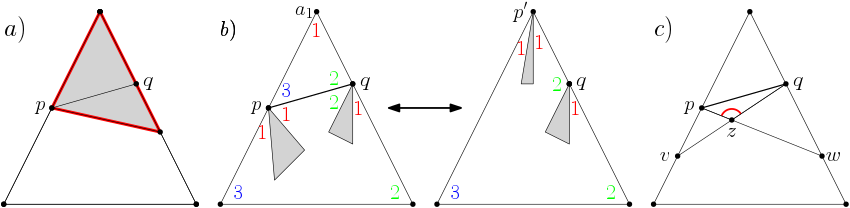
\includegraphics[width=0.9\textwidth]{lem3_1.png}
    	\caption{a) Unterteilendes Dreieck bei Grad 3. b) Kantenkontraktion der Kante $(a_1,p)$. c) Die Pfade die bei der Kontraktion von $(a_1,p)$ oder $(a_1,q)$ Degeneriertheit induzieren.}
    	\label{ccc1}
\end{figure}

Es kann also mindestens eine der Kanten kontrahiert werden. Sei $(a_1,p)$ diese Kante und $G'$ der Graph der durch Kontraktion von $(a_1,p)$ und das Löschen von $(p,q)$ entsteht. Wir erhalten das FAA $\phi'$ durch löschen der Zuweisung von $p$ aus $\phi$. Der Knoten $q$ ist weiterhin dem äusseren Gebiet zugewiesen. Da $G'$ weniger Knoten als $G$ hat ist er kein Gegenbeispiel und wir erhalten einen Schnyder Labeling $\sigma'$, das zusammen mit $\phi'$ ein Ecken kompatibles Paar bildet. Wir können $\phi'$ zu einem Labeling von $G$ erweitern indem wir, beginnend bei $a_1$, im Uhrzeigersinn die Label $1,2$ und $3$ im Gebiet $a_1,q,p$ einfügen. Wir erhalten ein Ecken kompatibles Paar. \\

\underline{2. Fall}: Sei $x$ der erste Nachbar von $p$ auf dem teilenden Segment. Wir Kontrahieren wieder die Kante $(a_1,p)$ um $G'$ zu erhalten. Bei der Kontraktion müssen keine weiteren Kanten gelöscht werden, wie in Abbildung \ref{pic_lem3_2} zu sehen ist. Wieder erhalten wir das FAA $\phi'$ auf $G'$ indem wir die Zuweisung von $p$ aus $\phi$ löschen. Zu jedem begrenzendem Pfad $\gamma$ in $G$, existiert $\gamma'$ in $G'$. Falls $x$ eine kombinatorisch konvexe Ecke einer der Zykel $\gamma$ ist, dann ist er dies auch für $\gamma'$, weil keine Kante an $x$ gelöscht wurde.

\begin{figure}[h]
	\centering
	  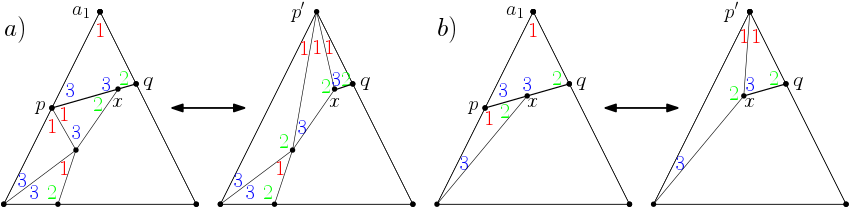
\includegraphics[width=0.9\textwidth]{lem3_2.png}
    	\caption{Zwei Beispiele zur Kontraktion von $(a_1,p)$ mit passendem Schnyder Labeling im zweiten Fall.}
    	\label{pic_lem3_2}
\end{figure}

Nun ist $G'$ kein Gegenbeispiel und es existiert ein zu $\phi'$ kompatibles Schnyder Labeling $\sigma'$. $\sigma'$ ist erweiterbar zu einem Labeling $\sigma$ für $G$. Füge Label 1 bei $a_1$ und 3 bei $p$ ein. $\Delta$ kann also kein teilendes Segment haben.

\end{proof}

Im nächsten Lemma wird eine Eigenschaft von Ecken kompatiblen Paaren festgehalten, die für den Beweis von Theorem \ref{theo_ccc} nützlich sein wird.

\begin{lemma}\label{lem4}
Sei G ein planer, intern-3-zusammenhängender Graph mit den Aufhängungen $\{a_1,a_2,a_3\}$ und einem Ecken kompatiblen Paar $(\sigma,\phi)$ aus einem Schnyder Labeling und einem FAA. Sei $v$ ein Nachbar einer Aufhängung $a_i$. Falls $v$ von $\phi$ einem Gebiet $f$ zugewiesen ist, das $a_i$ beinhaltet folgt, dass das Label von $v$ in $f$ nur einmal an $v$ vorkommt. Alle anderen Winkel an $v$ haben ein anderes Label.
\end{lemma}

\begin{proof}
Nehme ohne Beschränkung der Allgemeinheit an, dass $v$ ein Nachbar von $a_1$ ist und $v$ dem Gebiet $f$ auf der linken Seite der Kante $(a_1,v)$ zugeordnet ist (siehe Abbildung links). Sei $w$ der andere Nachbar von $v$ in $f$. 

\begin{minipage}{0.4\textwidth}
\begin{center}
    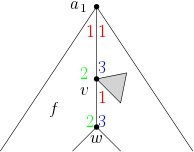
\includegraphics[width=0.9\textwidth]{lem4.png}
  \end{center}
\end{minipage}
\begin{minipage}{0.568\textwidth}
\vspace{1mm}
Die Kante $(a_1,v)$ hat zwei mal Label 1, jeweils links und rechts von $a_1$, und Label 2 am zugewiesenen Winkel von $v$. Nach Definition \ref{def_sl} muss an jeder Kante jedes Label einmal vorkommen. Somit ist das letzte Label an $(a_1,v)$ von Typ 3. Da $(\sigma,\phi)$ ein kompatibles Paar ist, muss der Winkel von $w$ in $f$ ebenfalls Label 2 haben, da sonst keine Ecke mit Label 2 existiert (vergleiche Definition \ref{def_sw}). Um die Kante $(v,w)$ müssen ebenfalls alle Label vorkommen und somit müssen wir 1 und 3 (wie in der Abbildung links) einfügen. 
\vspace{1mm}
\end{minipage}

Um $v$ existieren nach L2 im Uhrzeigersinn drei nichtleere Intervalle mit Label 1, 2 und 3. Folglich können die verbliebenen unbekannten Label an $v$ nur von Typ 1 oder 3 sein.
\end{proof}

\begin{lemma}\label{lem5}
In einem minimalen Gegenbeispiel $\Delta$, kann kein Nachbar $x_i$ einer der Aufhängungen $a_i$ einem Gebiet zugeordnet sein, zu dessen Rand die Kante $(a_i,x_i)$ gehört.
\end{lemma}

\begin{remark}
Lemma \ref{lem5} impliziert insbesondere, dass die drei Aufhängungen $a_1,a_2$ und $a_3$ von $\Delta$ ein Dreieck bilden.
\end{remark}

\begin{proof}
TODO
\end{proof}

\begin{lemma}\label{lem6}
Sei G ein planer, intern-3-zusammenhängender Graph mit den Aufhängungen $\{a_1,a_2,a_3\}$ der eine SLTR besitzt. Sei $\phi$ das von dieser SLTR induzierte FAA. Dann existiert ein Schnyder Labeling $\sigma$ von $G$, sodass $\sigma$ und $\phi$ ein Ecken kompatibles Paar bilden.
\end{lemma}

\begin{proof}
Angenommen das Lemma gilt nicht und sei $G$ ein minimales Gegenbeispiel, wie zuvor mit der minimalen Anzahl an Knoten und unter diesen mit der minimalen Anzahl an Kanten. Sei $\Delta$ eine SLTR von $G$ mit den Aufhängungen $a_1,a_2,a_3$ und $\phi$ das induzierte FAA. Wir wollen wieder zu einem Widersprich gelangen indem wir einen kleineren Graphen $G'$ konstruieren, sodass die folgenden Punkte erfüllt sind.
\begin{itemize}
\item $G'$ besitzt ein FAA $\phi'$, welches von $\phi$ indiziert wird.
\item Das kompatible Paar $(\sigma',\phi')$ von $G'$ induziert ein Schnyder Labeling von $G$.
\item Das so erzeugte Schnyder Labeling $\sigma$ ist Ecken kompatibel zu $\phi$.
\end{itemize}
Diese Aussagen zusammen erzeugen einen Widerspruch zur Annahme, dass $G$ ein Gegenbeispiel ist. Wir halten einige Beobachtungen aus den vorherigen Lemmata fest.
\begin{itemize}
\item [B1] $\Delta$ hat kein unterteilendes Dreieck.
\item [B2] $\Delta$ hat kein teilendes Segment und somit keine Aufhängung von Grad 2.
\item [B3] Kein Nachbar $x_i$ einer Aufhängung $a_i$ kann einem Gebiet zugeordnet sein, zu dessen Rand die Kante $(a_i,x_i)$ gehört. Somit bilden die Aufhängungen von $\Delta$ ein Dreieck.
\end{itemize}

Aus B3 folgt, dass sowohl das äussere Gebiet als auch seine drei benachbarten Gebiete (echte) Dreiecke\footnote{Sie enthalten nur jeweils ihre drei Ecken als Knoten.} sind (siehe Abbildung \ref{pic_lem6_1} links). Wir werden sehen, dass der dritte Knoten in einem der inneren Dreiecke eine wichtige Rolle spielt. Wir bezeichnen den dritten Knoten im Dreieck, das $a_i$ und $a_{i+1}$ enthält, mit $q_i$ (oder einfach nur $q$).

Der Beweis läuft in drei Schritten. Wir zeigen zuerst, dass in einem minimalen Gegenbeispiel $\Delta$ jedes $q_i$ einem angrenzenden Gebiet zugeordnet sein muss (und in diesem einen flachen Winkel hat). Falls dies gilt, zeigen wir, dass wir aus $G$ einen Graphen $G'$ erzeugen können, der einen zugewiesenen Knoten $q'$ auf einer Kante $(a_i,q')$ besitzt und erhalten einen Widerspruch zu B3. Zuletzt zeigen wir, dass wir aus einem Schnyder Labeling $\sigma'$ von $G'$ ein Labeling $\sigma$ von $G$ erzeugen können, sodass aus der Ecken Kompatibilität von $\sigma'$ und $\phi'$ auch Kompatibilität von $\sigma$ und $\phi$ folgt.

\begin{figure}
	\centering
	  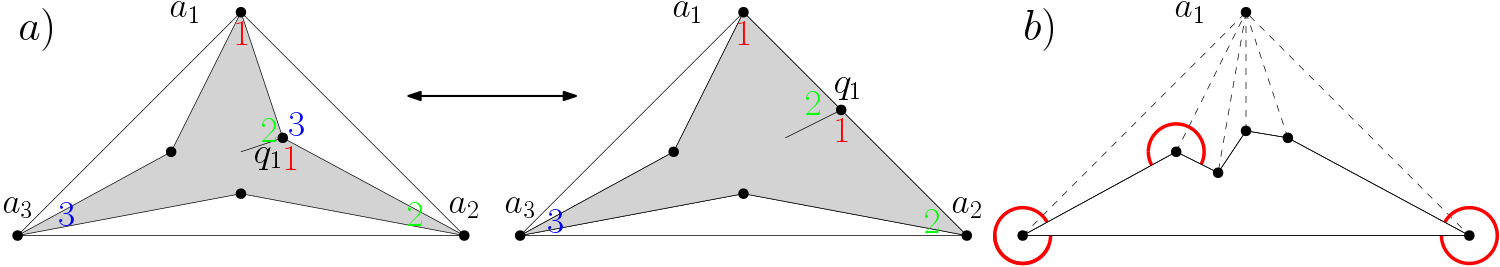
\includegraphics[width=0.9\textwidth]{lem6_1.png}
    	\caption{a) Die Erstellung eines Graphen $G'$ mit weniger Kanten. b) Das Löschen einer Aufhängung resultiert in einem Graphen mit mindestens drei Aussenwinkeln $\geq \pi$.}
    	\label{pic_lem6_1}
\end{figure}

Sei $f$ das von $a_1,a_2$ und $q_1$ gebildete Dreieck (siehe Abbildung \ref{pic_lem6_1}, a)). Angenommen $q_1$ wird von $\phi$ nicht zugeordnet. Entferne die Kante $(a_1,a_2)$ und weise $q_1$ in dem äusseren Gebiet zu, um $G'$ und $\sigma'$ zu erhalten. Kein begrenzender Zykel enthält den neu zugewiesenen Winkel an $q$ in seinem Inneren. Falls $a_1$ und $a_2$ auf einem begrenzenden Zykel $\gamma'$ liegen, dann ist $q$ keine Ecke des korrespondierenden Zykels $\gamma$ in $G$ sein, sondern muss in seinem Inneren liegen (sonst wäre $\gamma'$ von einem Pfad induziert). Somit sind die kombinatorisch konvexen Ecken von $\gamma$ ebensolche von $\gamma$. Da Zykel die $q$ nicht enthalten keine Ecken verlieren, hat jeder begrenzende Zykel in $G'$ mindestens drei kombinatorisch konvexe Ecken. Somit hat $G'$ ein SLTR $\Delta'$ und die gerade Winkel werden von $\phi'$ induziert. Nun ist $G'$ ein Graph mit weniger Kanten als $G$ und somit kein Gegenbeispiel. Wir erhalten also ein Ecken kompatibles Paar $(\sigma',\phi')$. Wir können dies wie in Abbildung \ref{pic_lem6_1} zu einem Paar für $G$ erweitern.

Nehmen wir also an, dass jedes der $q_i$ in einem Gebiet einen flachen Winkel hat, also von $\phi$ einem Gebiet zugeordnet wird. Jede Aufhängung $a_i$ muss mindestens einen Nachbarn $x_i$ haben, der nicht zugeordnet ist. Wäre dies nicht der Fall, dann entstünde ein Widerspruch zur Tatsache, dass $G\backslash \{a_1\}$ drei konkave Aussenwinkel hat (siehe Abbildung \ref{pic_lem6_1}, b)). Der Knoten mit Winkel $\geq \pi$, der keine Aufhängung ist, kann zuvor nicht zugeordnet sein. Sei nun ohne Beschränkung der Allgemeinheit $q$ gemeinsame Nachbar von $a_1$ und $a_2$. $p_k$ sei der im Uhrzeigersinn von $q$ ausgehend erste Nachbar von $a_1$ der nicht zugewiesen ist (In Abbildung \ref{pic_lem6_2} ist dies $p_3$).

Wir werden einen Graphen $G'$ (mit der gleichen Anzahl an Knoten und weniger Kanten) aus $G$ erstellen. In diesem Graphen ist $p_k$ einem Gebiet zugeordnet, auf dessen Rand die Kante $(a_1,p_k)$ liegt. Nach Lemma \ref{lem5} muss somit ein Schnyder Labeling $\sigma'$ existieren, dass Ecken kompatibel mit dem induzierten FAA $\phi'$ von $G'$ ist. Wir können aus $\sigma'$ ein Schnyder Labeling $\sigma$ für $G$ bauen, dass kompatibel zu $\phi$ ist.

Sei $N_{a_1} = \{q,p_1,\ldots,p_k,\ldots,p_l,a_3,a_2\}$ die Menge der Nachbarn von $a_1$, wobei wir mit $q$ beginnen und im Uhrzeigersinn fortfahren. Durch löschen der Kante $(a_1,q)$ und einfügen der Kante $(a_2,p_1)$ erhalten wir einen neuen Graphen $G_1$. Wir nennen den durchgeführten Kantenwechsel um $G_1$ zu erhalten (nach dem Englischen) einen \textit{flip}. $G_1$ lässt die SLTR $\Delta_1$ zu. Die vier Knoten $a_1,a_2,q$ und $p$ bilden in $\Delta$ ein konvexes Viereck\footnote{Auf der Geraden zwischen $q$ und $p_1$ können sich zusätzliche Knoten befinden, doch dies spielt für unsere Argumentation keine Rolle.} mit nur einer Diagonalen im Inneren (vergleiche Abbildung \ref{pic_lem6_2}, a) und b)). Die erhaltene Zeichnung $\Delta_1$ ist somit ebenfalls eine SLTR. Falls $p_1$ zugewiesen ist, wiederholen wir den Schritt (siehe Abbildung \ref{pic_lem6_2}, c)). Wir führen diesen Schritt nur so oft durch, bis wir bei $p_k$ angekommen sind, dem ersten nicht zugewiesenen Nachbar von $a_1$, und die Diagonale im konvexen Viereck $a_1,a_2,p_{k-1},p_k$ flippen. Wir ersetzen also $(a_1,p_{k-1})$ durch $(a_2,p_{k})$. Nach jedem \textit{flip} erhalten wir ein SLTR $\Delta_i$ von $G_i$ und somit ist $\phi_k$ ein Gutes-FAA.

\begin{figure}
	\centering
	  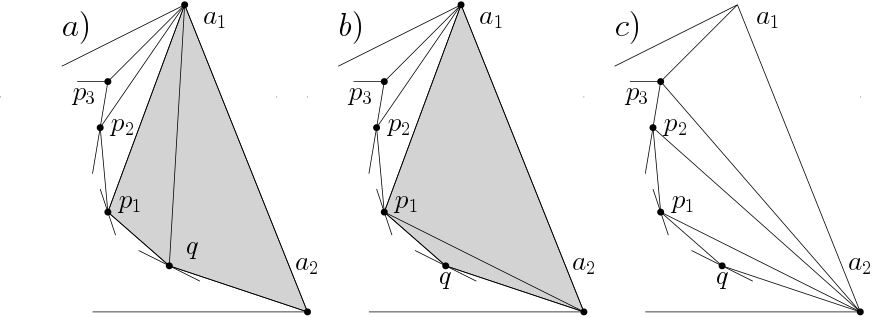
\includegraphics[width=0.9\textwidth]{lem6_2.png}
    	\caption{Das schrittweise Flippen von Kanten.}
    	\label{pic_lem6_2}
\end{figure}

Um nun den Graphen $G'$ zu erhalten löschen wir die im letzten \textit{flip} hinzugefügte Kante $(a_2,p_{k})$ (siehe Abbildung \ref{pic_lem6_3}, b)). $G'$ hat somit eine Kante weniger als $G$. $p_k$ ist in $\phi_k$ nicht zugewiesen. Sei $\phi'$ der Erweiterung von $\phi_k$ um die Zuweisung von $p_k$ zum Gebiet $a_1,a_2,p_{k-1},p_k$ (siehe Abbildung \ref{pic_lem6_3}, a)). Dann ist $\phi'$ ein FAA von $G'$. Wir zeigen als Nächstes, dass es sich bei $\phi'$ um ein Gutes-FAA handelt.

Betrachten wir einen beliebigen begrenzenden Zykel $\gamma'$ in $G'$ und sei $\gamma_k$ der korrespondierende Zykel in $G_k$ Wir müssen wieder zeigen, dass jeder Zykel mindestens drei kombinatorisch konvexe Ecken hat. Im Fall, dass $p_k$ nicht auf dem Rand von $\gamma'$ liegt, folgt sofort, dass beide Zykel die selben kombinatorisch konvexen Ecken haben (und somit beide mindestens drei). Betrachten wir also den Fall, dass $p_k$ auf dem Rand von $\gamma'$ liegt. Im Fall, dass $\gamma'$ nur einen Teil der Nachbarn von $p_k$ beinhaltet und nicht den zugewiesenen Winkel einschließt ist $p_k$ sowohl eine kombinatorisch konvexe Ecke von $\gamma_k$ und somit auch von $\gamma'$. Sei also $p_k$ keine kombinatorisch konvexe Ecke von $\gamma'$. Falls der zugewiesene Winkel an $p_k$ im Inneren von $\gamma'$ liegt, aber $\gamma'$ nicht alle Nachbarn von $p_k$ enthält, muss $\gamma_k$ mindestens vier kombinatorisch konvexe Ecken besitzen. Die ersten drei sind $a_1,a_2$ und $p_k$ und die vierte befindet sich auf dem Teil des Randes $R$ vom $\gamma'$ zwischen $p_k$ und $a_2$\footnote{Diese Ecke muss existieren, da der begrenzende Zykel $\tilde{\gamma}$, der sich aus $R$ und der Kante $(a_2,p_k)$ bildet, mindestens drei kombinatorisch konvexe Ecken in $G_k$ hat.}. Somit hat $\gamma'$ mindestens drei kombinatorisch konvexe Ecken. Betrachte den Fall, dass $\gamma'$ alle Nachbarn von $p_k$ beinhaltet, aber der zugewiesene Winkel nicht im Inneren von $\gamma'$ liegt. In der SLTR $\Delta_k$ ist der Aussenwinkel von $\gamma_k$ am Knoten $p_k$ somit nicht grösser als $\pi$ und $\gamma_k$ muss drei andere (kombinatorisch konvexe) Ecken haben. Diese sind auch kombinatorisch konvexe) Ecken von $\gamma'$. Somit hat jeder begrenzende Zykel $\gamma'$ in $G'$ mindestens drei kombinatorisch konvexe Ecken und es folgt, dass $\phi'$ ein Gutes-FAA ist.

Da $G'$ die gleiche Anzahl an Knoten und weniger Kanten als $G$ kann er kein Gegenbeispiel sein. Es existiert also ein Schnyder Labeling $\sigma'$, das Ecken kompatibel zu $\phi'$ ist. Es bleibt zu zeigen, dass wir aus $\sigma'$ ein Labeling für $G$ erstellen können, welches dann Ecken kompatibel zu $\phi$ ist. Wir stützen uns hierfür auf die folgende Eigenschaft, die aus C2 folgt.

\begin{itemize} 
\item [C3] In einem Ecken kompatiblen Paar $(\sigma,\phi)$ hat jeder zugewiesene Winkel in diesem Gebiet (mindestens) einen benachbarten Winkel mit dem selben Label.
\end{itemize}

\begin{figure}
	\centering
	  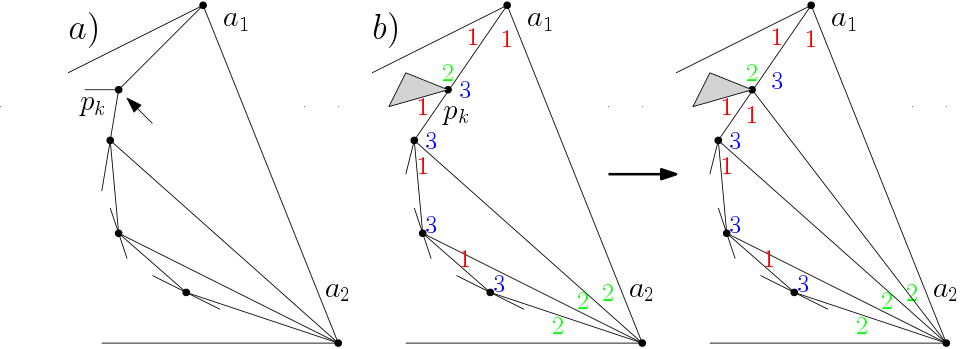
\includegraphics[width=0.9\textwidth]{lem6_3.png}
    	\caption{Ein Schnyder Labeling von $G_k$ erstellt aus einem Labeling von $G'$. }
    	\label{pic_lem6_3}
\end{figure}

Das Schnyder Labeling $\sigma'$ ist eindeutig für Gebiete (TODO) mit $a_1$ oder $a_2$ als Ecken und einer geflippten Kante auf dem Rand (siehe Abbildung \ref{pic_lem6_3}, b)). In einem ersten Schritt müssen wir $(a_2,p_k)$ wieder einfügen und $\sigma'$ eindeutig erweitern (wie in Abbildung \ref{pic_lem6_3} b) zu sehen).

Die Flips wurden entlang $q,p_1,\ldots,p_k$ durchgeführt und nach unserer Annahme haben die Knoten $p_1,\ldots,p_{k-1}$ von $\phi'$ zugewiesene Winkel in $G'$. Sei $p_0$=$q$. Zwei Knoten $p_{i-1}$ und $p_i$, mit $i \in \{1,\ldots,k\}$ in dieser Folge sind nicht zwangsläufig Nachbarn, aber sie sind die Ecken des (dreieckigen) Gebietes $a_2,p_{i-1},p_{i}$ und alle Knoten auf dem Rand zwischen $p_{i-1}$ und $p_{i}$ sind diesem Gebiet zugewiesen (siehe Abbildung \ref{pic_lem6_4}, a)). Wir führen nun Schritt für Schritt, beginnend mit $i=k$, einen \textit{rückwärts flip} durch. Hierfür entfernen wir die Kante $(p_{i},a_2)$ wieder und setzen die Kante $(p_{i},a_1)$ wieder ein. Merke, dass $p_{i}$ vor dem Schritt $i$ einen zusätzlichen Nachbarn in $G_{i}$ (im Verhältnis zu $G$) hat und somit gilt $deg(p_{i}) \geq 4$, weil $G$ intern-3-zusammenhängend ist. Sei $\alpha_{i}$ der gegen den Uhrzeigersinn auf die Kante zu $a_1$ folgende Winkel und $\beta_{i}$ der im Uhrzeigersinn auf die Kante zu $p_{i-1}$ folgende Winkel (jeweils an $p_{i}$). Dann handelt es sich bei diesen Winkeln, wegen $deg(p_i) \geq 4$, nicht um den Selben. Bei jedem Schritt wird die folgende Invariante eingehalten.

\begin{invariant}
Vor dem Schritt $i$ hat der Knoten $p_i$ die Label 2,3,1,1 im Uhrzeigersinn beginnend mit den Winkel $\alpha_i$ und Enden mit $\beta_i$ (siehe Abbildung \ref{pic_lem6_4}, a)). Zusätzlich bilden das Schnyder Labeling $\sigma'_i$ und das FAA $\phi'_i$ ein Ecken kompatibles Paar auf $G'_i$.
\end{invariant}

Beginnen wir mit $G'$. Hier sind die in Abbildung \ref{pic_lem6_3} b) gewählten Label der Winkel um $p_k$ die einzig mögliche Kombination. Genauso verhält es sich nach dem Einfügen der Kante $(a_2,p_k)$. Wir erhalten den Graphen $G'_{k}, das Schnyder Labeling \sigma'_{k}$ und das FAA $\phi'_{k}$, wobei $\sigma'_{k}$ und $\phi'_{k}$ ein Ecken kompatibles Paar bilden. Somit gilt die Invariante vor dem ersten Schritt.

Die Invariante gelte vor Schritt $i$. In Schritt $i$ entfernen wir die Kante $(a_2,p_i)$ und fügen die Kante $(a_1,p_{i-1})$ wieder in den Graphen ein. Vor dem \textit{rückwärts flip}, erfüllen die Label um $p_i$ die Invariante und $\sigma'_{i}$ und $\phi'_{i}$ sind ein Ecken kompatibles Paar. Die folgende Argumentation basiert auf Lemma \ref{lem_sl} -- die Kanten Regel besagt, dass alle drei Label im Uhrzeigersinn an jeder Kante vorkommen -- und der Ecken Kompatibilität von $(\sigma'_{i},\phi'_{i})$. Die Winkel an $p_{i-1}$ links und rechts der Kante zu $p_i$ haben die Label 2 und 3 (siehe Abbildung \ref{pic_lem6_4}, b)). Der Winkel zwischen $p_i$ und $a_2$ kann nur Label 3 haben, da er an einer Kante zu $a_2$ liegt, an deren anderem Ende somit nur Label 2 vorkommt. Der andere Winkel muss Label 2 haben, da er entweder an einer Kante mit zwei 3ern auf der anderen Seite liegt (vergleiche Abbildung \ref{pic_lem6_4}, a)) oder er an der Kante $(p_i,p_{i-1})$ liegt, nur mir Label 1 an $p_i$ (vergleiche Abbildung \ref{pic_lem6_4} Mitte). 

\begin{figure}
	\centering
	  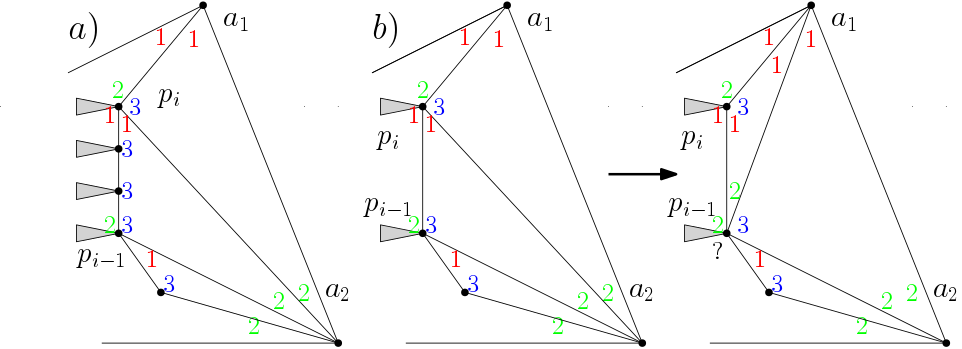
\includegraphics[width=0.9\textwidth]{lem6_4.png}
    	\caption{a) Schnyder Labeling zwischen $p_{i-1}$ und $p_{i}$. b) Änderung des Labelings beim rückwärts Flippen.}
    	\label{pic_lem6_4}
\end{figure}

Führen wir den \textit{rückwärts flip} durch. Wir löschen also die Kante $(a_2,p_i)$ und fügen die Kante $(a_1,p_{i-1})$ ein, wie in Abbildung \ref{pic_lem6_4} b). Für fast alle Winkel folgt die Wahl des Labels eindeutig, da $\sigma'_{i-1}$ ein Schnyder Labeling sein muss. Um die Invariante zu erfüllen müssen wir zeigen, dass wir dem mit ? markierte Winkel Label 1 geben können. Wenn er diese Label schon vor dem Schritt hatte ändert sich nichts und wir sind fertig. Angenommen er hatte nicht Label 1. Da es sich um ein Schnyder Labeling handelt ist die einzig andere Möglichkeit Label 2. Es muss sich bei diesem Winkel, um den an $p_{i-1}$ zugewiesenen handeln. Dies folgt aus der Ecken Kompatibilität, da ein zugewiesener Winkel und seine beiden Nachbarn um einen Knoten nicht alle die gleichen Label haben können. Sonst kommt es, wie in Abbildung \ref{pic_lem6_5} a), zu einem Widerspruch, weil alle weiteren Winkel an $p_{i-1}$ Label 2 haben und so ein Gebiet keine Ecke mit diesem Label hätte.

\begin{figure}[h]
	\centering
	  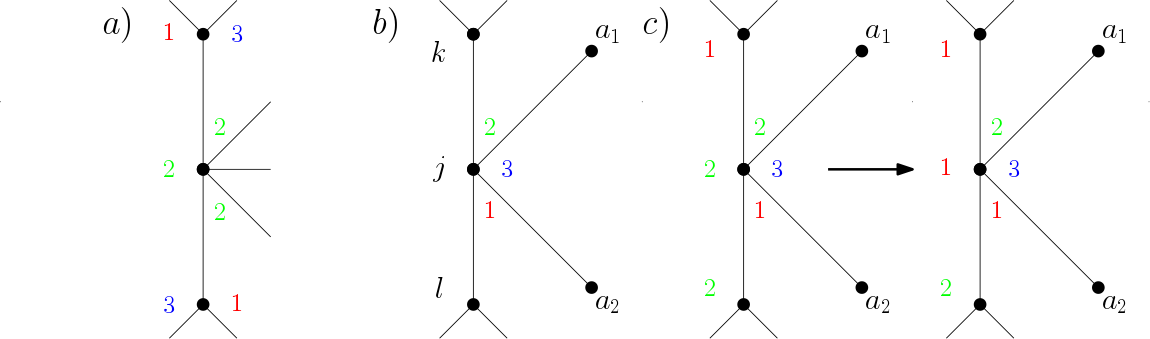
\includegraphics[width=0.8\textwidth]{lem6_5.png}
    	\caption{a) Das Gebiet links kann keine Ecke mit Label 1 haben.}
    	\label{pic_lem6_5}
\end{figure}

Betrachte Abbildung \ref{pic_lem6_5} b). Wenn wir $j$=2 setzten, dann folgen sofort die Label in c). $j$=2 folgt aus der Kanten Regel (Lemma \ref{lem_sl}). Nun muss $l$=2 sein, weil sonst das Gebiet auf der linken Seite keine Ecke mit Label 2 haben könnte. Wir können also das Label auf 1 setzten und erhalten ein Schnyder Labeling $\sigma'_{i-1}$ (siehe Abbildung \ref{pic_lem6_5}, c)), das Ecken kompatibel mit dem induzierten FAA $\phi'_{i-1}$ ist, da wir nur das Label eines zugewiesen Winkels verändert haben.

Wir haben also Schritt $i$ durchgeführt und die Invariante hat bestand. Per Induktion erhalten wir ein Ecken kompatibles Paar aus einem Schnyder Labeling $\sigma'_0$ und einem FAA $\phi'_0$ von $G$. Somit kann $G$ kein Gegenbeispiel sein. Es folgt die Rückrichtung des Theorems.
\end{proof}

Wir haben nun alle nötigen Hilfsmittel um Theorem \ref{theo_ccc} zu beweisen. 

\begin{proof}[Beweis von Theorem \ref{theo_ccc}]
Sei G ein planer, intern-3-zusammenhängender Graph mit den Aufhängungen $\{a_1,a_2,a_3\}$. Angenommen $G$ besitzt ein Ecken kompatibles Paar $(\sigma,\phi)$ aus einem Schnyder Labeling $\sigma$ und einem FAA $\phi$. Nach Lemma \ref{lem1} existiert dann eine SLTR von $G$. 

Angenommen $G$ besitzt eine SLTR, dann existert nach Lemma \ref{lem6} ein Schnyder Labeling, das Ecken kompatibel mit dem von der SLTR induzierten FAA ist.
\end{proof}







